\documentclass[usenames,dvipsnames]{beamer}

\mode<presentation> {
\usetheme{Montpellier}
}

\usepackage{graphicx}
\usepackage{booktabs}
\usepackage[utf8]{inputenc}
\setcounter{tocdepth}{2}
\graphicspath{{../../Figures/}}


% exercices comptés
\newcounter{numexos}%Création d'un compteur qui s'appelle numexos
\setcounter{numexos}{0}%initialisation du compteur
\newcommand{\exercice}[1]{%Création d'une macro ayant un paramètre
\addtocounter{numexos}{1}%chaque fois que cette macro est appelée, elle ajoute 1 au compteur numexos
\textcolor{DarkOrchid}{Exercice\,\thenumexos\,:}\,#1%Met en rouge Exercice et la valeur du compteur appelée par \thenumeexos
}

%----------------------------------------------------------------------------------------
%	TITLE PAGE
%----------------------------------------------------------------------------------------

\setbeamertemplate{title page}{
    \centering

    \Large\bfseries
    Machine learning Tek 5: neural networks
    

\begin{figure}[!h]

\includegraphics[width=8cm]{learning_rates_overparametrized}
\end{figure}

    }
\begin{document}

\begin{frame}
\titlepage 
\end{frame}

\begin{frame}
    \begin{figure}[htpb]
        \centering
        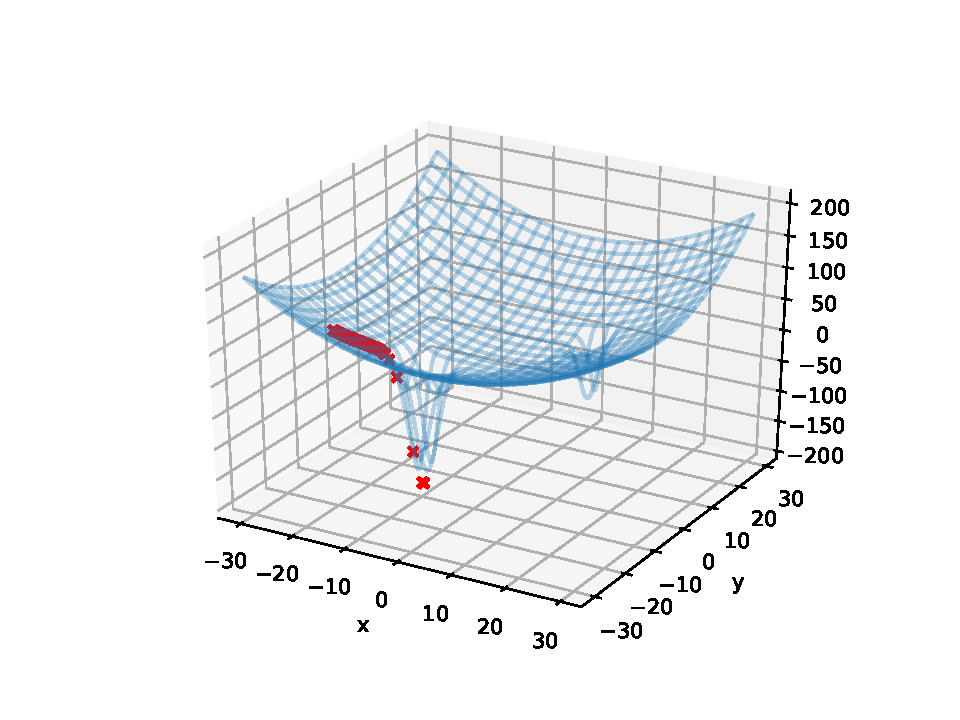
\includegraphics[width=0.94\linewidth]{47500}
        \label{fig:47500}
    \end{figure}
    
\end{frame}

\begin{frame}
    \tableofcontents
\end{frame}

\begin{frame}{Ressources}
    \begin{itemize}
        \item \url{https://www.deeplearningbook.org/} 
	\item \url{https://course.fast.ai/} 
        \item \url{https://d2l.ai/} 
        \item \url{https://mlelarge.github.io/dataflowr-web/dldiy_ens.html} 
        \item \url{https://playground.tensorflow.org/} 
        \item \url{http://www.jzliu.net/blog/simple-python-library-visualize-neural-network/} 
    \end{itemize}
\end{frame}

\section{Vectors, matrices, neural nets}%
\label{sec:vectors_matrices_neural_nets}

\begin{frame}
\frametitle{Elementary neuron}
    A \textbf{{neuron}} is a \textbf{{mapping}} from a multidimensional input
    $x=(x_1,...,x_d)$ to a real number.

    This function depends on \textbf{{parameters}} called the \textbf{{weights}}
    $w=(w_1,...,w_d)$ and the \textbf{intercept} $b$ (omitted in the following slides to simplify the notations).

    \begin{equation}
	f(x)=\sigma( \sum^{d}_{i=1} x_iw_i )
    \end{equation}
Where $\sigma$ is a non linear function, for instance a \textbf{{sigmoid}}.
\end{frame}

\begin{frame}{Sigmoid function}
   \begin{figure}[htpb]
       \centering
       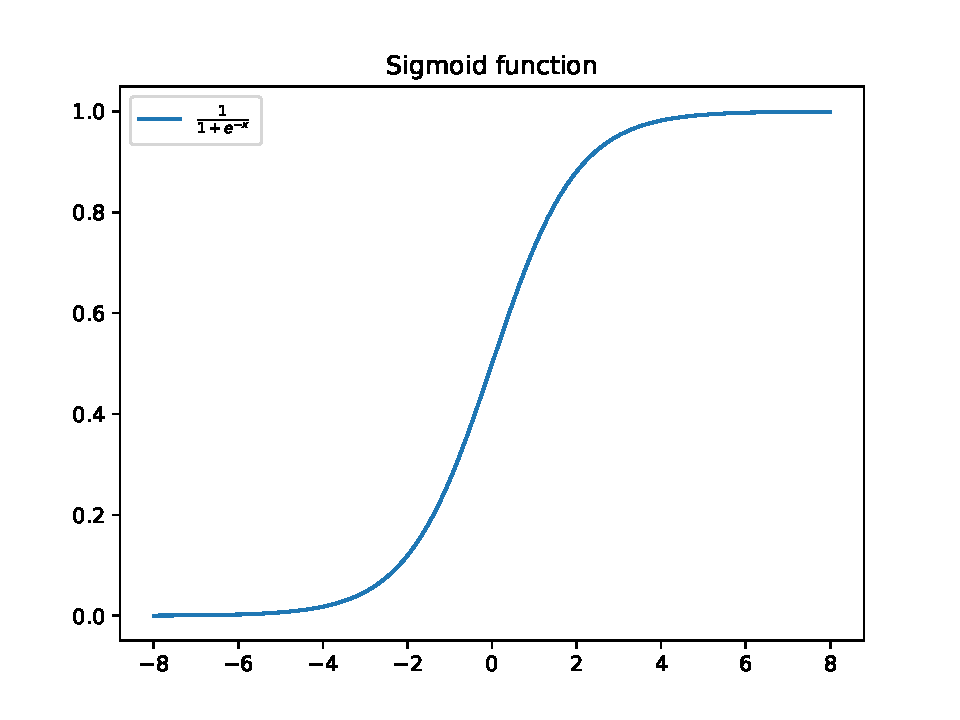
\includegraphics[width=0.8\linewidth]{sigmoid}
       \label{fig:sigmoid}
   \end{figure} 
\end{frame}


\begin{frame}{Sigmoid function}
   \begin{figure}[htpb]
       \centering
       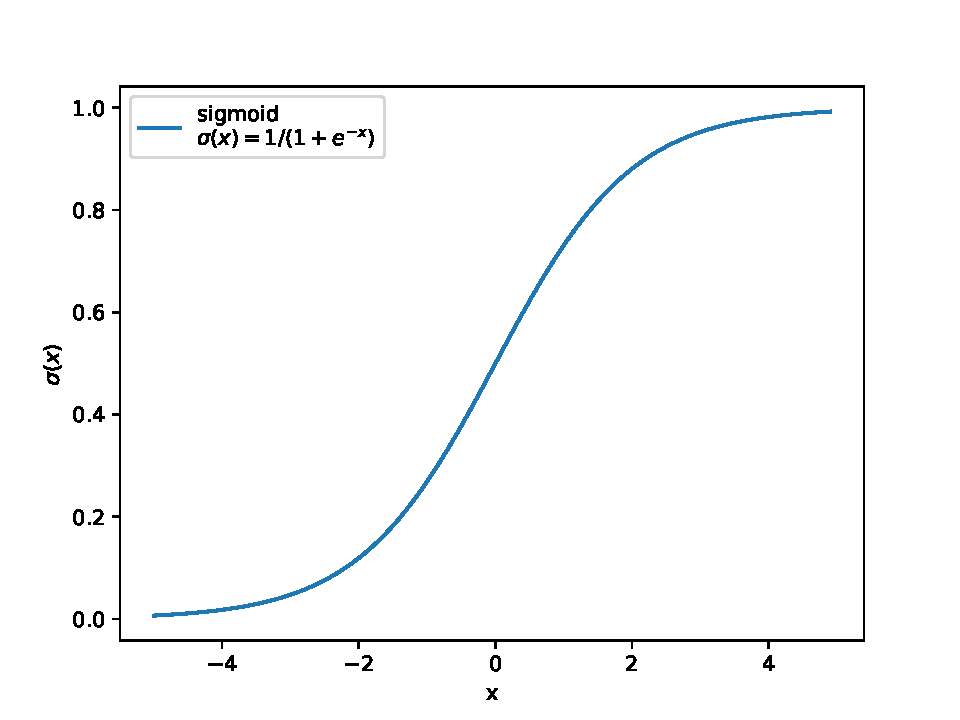
\includegraphics[width=0.8\linewidth]{sigmoid_zoom_in}
       \label{fig:sigmoid}
   \end{figure} 
\end{frame}


\begin{frame}{Sigmoid function}
   \begin{figure}[htpb]
       \centering
       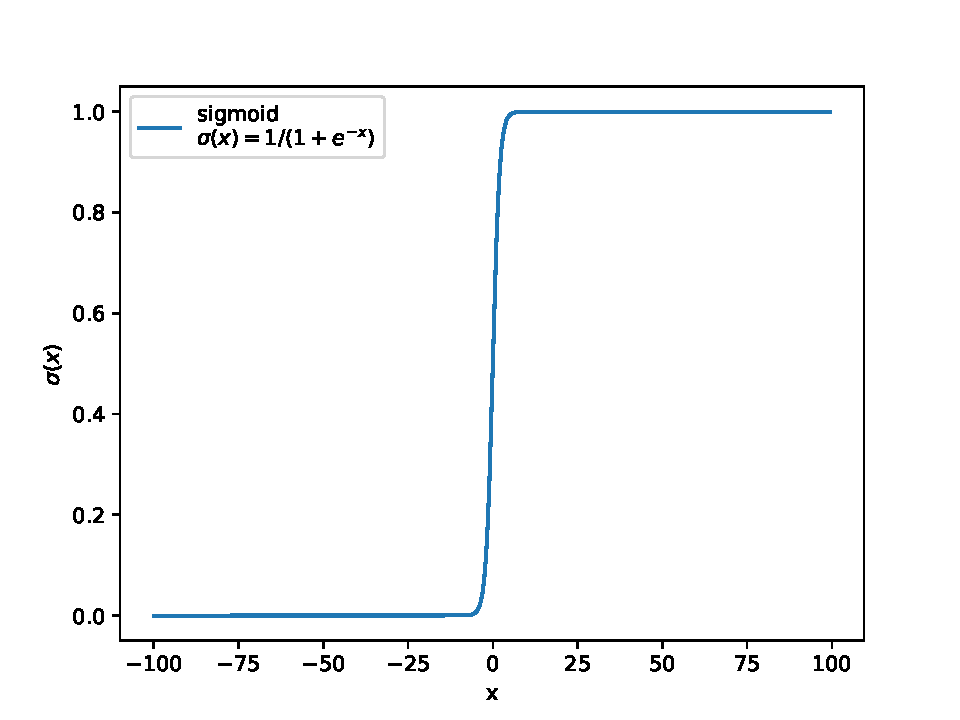
\includegraphics[width=0.8\linewidth]{sigmoid_zoom_out}
       \label{fig:sigmoid}
   \end{figure} 
\end{frame}

\begin{frame}{Notation with vectors}
    The sum $   \sum^{d}_{i=1} x_iw_i  $ can also be written this way : 
    \begin{equation}
        xw^T
    \end{equation}
    This means a \textbf{{product}} of \textbf{{two matrices}} (a vector is
    also a matrix : it is just a matrix with only one line or only one column): 
    \begin{itemize}
       \item $x=(x_1,...,x_d)$
                \item 
$$
w^T=
\begin{pmatrix}
w_1\\
w_2\\
\vdots\\
w_d
\end{pmatrix}
$$
    \end{itemize}
\end{frame}

\begin{frame}{Matrices}
    A matrix is an array used to store data. It has \textbf{{lines}}  and
    \textbf{{columns}} 
$$
A=
\begin{pmatrix}
1 & 4 & 1 \\
0 & 1 & 2 \\
0 & 0 & 1
\end{pmatrix}
$$
    $A_{ij}$ means the element at line $i$ and column $j$.
    \begin{itemize}
        \item $A_{12}=4$
        \item $A_{31}=0$
        \item $A_{33}=1$
    \end{itemize}
\end{frame}

\begin{frame}{Matricial multiplication}
    \begin{itemize}
        \item If matrix $A$ has $p$ columns and matrix $B$ has $p$ lines, the
            product $AB$ of the two matrices is defined as:
            \begin{equation}
                AB_{ij}= \sum^{p}_{k=1} A_{ik}B_{kj}
            \end{equation}
	\item \url{https://en.wikipedia.org/wiki/Matrix_multiplication}
        \item It is often more convenient and compact to write computations as operations on vectors and matrices when possible.
    \end{itemize}
\end{frame}

\begin{frame}{Examples}
   \[
\begin{pmatrix}
1 & 4 & 1 \\
0 & 1 & 2 \\
0 & 0 & 1
\end{pmatrix}
\begin{pmatrix}
0 & 0 & 0 \\
0 & 0 & 0 \\
0 & 0 & 0
\end{pmatrix}
    =\text{?} 
\] 
\end{frame}

\begin{frame}{Examples}
   \[
\begin{pmatrix}
1 & 4 & 1 \\
0 & 1 & 2 \\
0 & 0 & 1
\end{pmatrix}
\begin{pmatrix}
0 & 0 & 0 \\
0 & 0 & 0 \\
0 & 0 & 0
\end{pmatrix}
    =
\begin{pmatrix}
0 & 0 & 0 \\
0 & 0 & 0 \\
0 & 0 & 0
\end{pmatrix}
\] 
\end{frame}


\begin{frame}{Examples}
   \[
\begin{pmatrix}
1 & 4 & 1 \\
0 & 1 & 2 \\
0 & 0 & 1
\end{pmatrix}
\begin{pmatrix}
1 & 0 & 0 \\
0 & 1 & 0 \\
0 & 0 & 1
\end{pmatrix}
    =\text{?} 
\] 
\end{frame}

\begin{frame}{Examples}
   \[
\begin{pmatrix}
1 & 4 & 1 \\
0 & 1 & 2 \\
0 & 0 & 1
\end{pmatrix}
\begin{pmatrix}
1 & 0 & 0 \\
0 & 1 & 0 \\
0 & 0 & 1
\end{pmatrix}
    =
\begin{pmatrix}
1 & 4 & 1 \\
0 & 1 & 2 \\
0 & 0 & 1
\end{pmatrix}
\] 
\end{frame}



\begin{frame}{Examples}
   \[
\begin{pmatrix}
1 & 4 & 1 \\
0 & 1 & 2 \\
0 & 0 & 1
\end{pmatrix}
\begin{pmatrix}
1 & 0 & 0 \\
0 & 2 & 0 \\
1 & 0 & 0
\end{pmatrix}
    =\text{?} 
\] 
\end{frame}

\begin{frame}{Examples}
   \[
\begin{pmatrix}
1 & 4 & 1 \\
0 & 1 & 2 \\
0 & 0 & 1
\end{pmatrix}
\begin{pmatrix}
1 & 0 & 0 \\
0 & 2 & 0 \\
1 & 0 & 0
\end{pmatrix}
    =
\begin{pmatrix}
2 & 8 & 0 \\
2 & 2 & 0 \\
1 & 0 & 0
\end{pmatrix}
\] 
\end{frame}


\begin{frame}{Examples}
   \[A=
\begin{pmatrix}
1 & 1 & 1 \\
1 & 1 & 1 \\
1 & 1 & 1
\end{pmatrix}
\] 
What is $A^n$ ?
\end{frame}

\begin{frame}{Examples}
    \begin{itemize}
        \item $x=(x_1,...,x_d)$
        \item $w=(w_1,...,w_d)$
    \end{itemize}
    \begin{equation}
    xw^T= \sum^{d}_{i=1} x_iw_i
    \end{equation}
\end{frame}

\begin{frame}{Neural networks}
    \begin{itemize}
        \item $\sigma(xw^T )$ allows us to compute the output of a
            \textbf{{single neuron}} 
        \item But we will often have \textbf{{several neurons}} outputting a
            result.
        \item These neurons are organized in a network called neural network.
    \end{itemize}
\end{frame}

\begin{frame}
    \begin{itemize}
        \item Let $w=[w_{ij}]$ be the matrices of weights between neuron $i$ of
            the left layer and neuron $j$ of the middle layer.
            \begin{figure}[htpb]
                \centering
                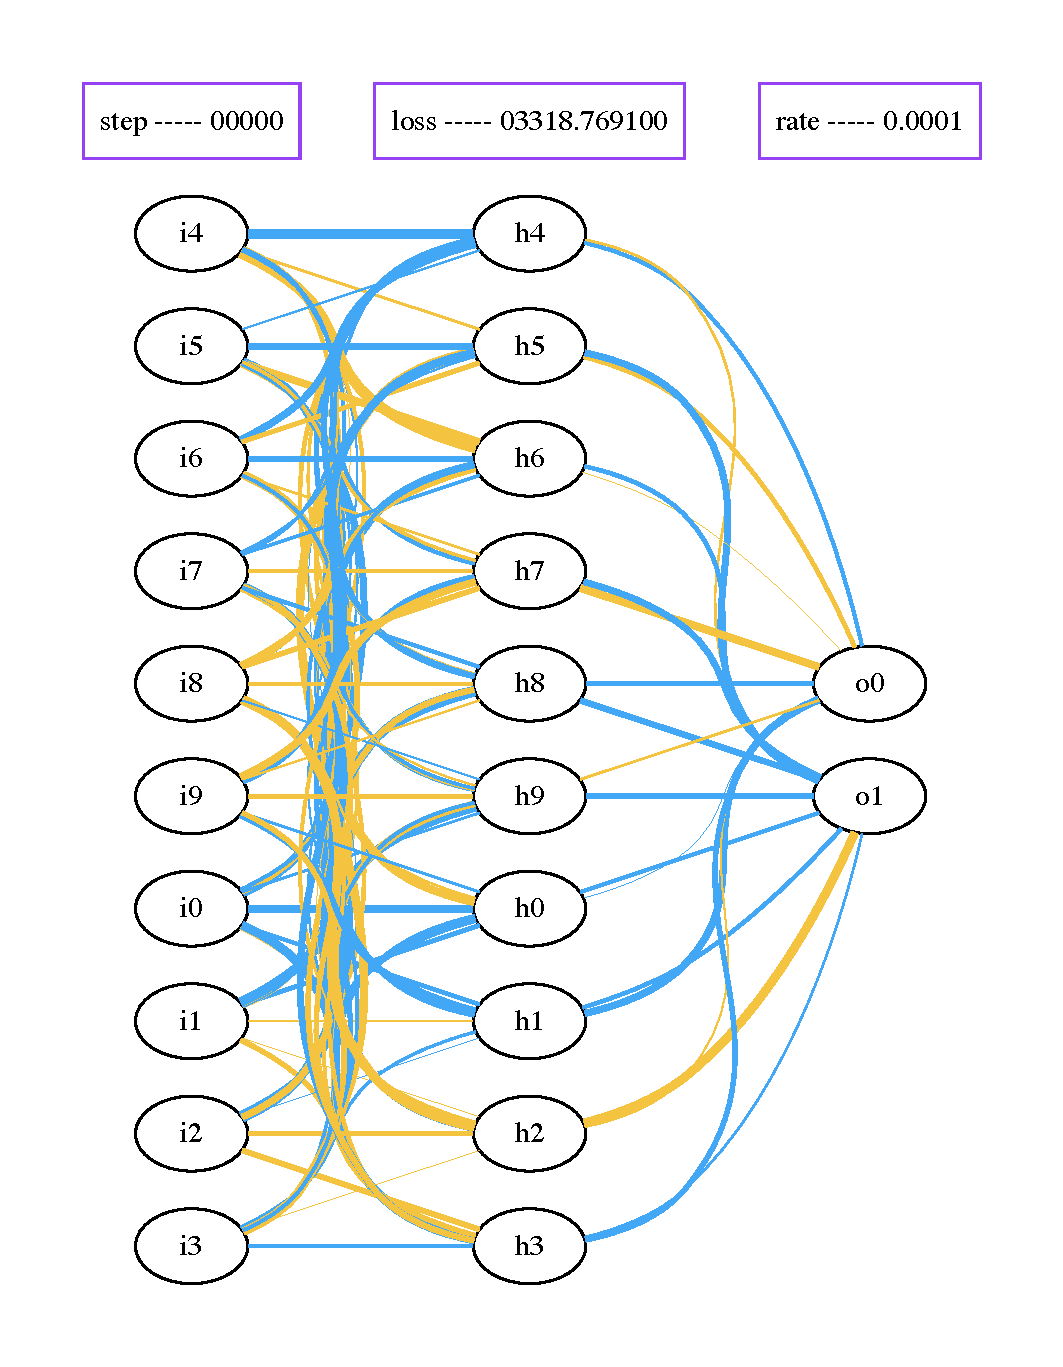
\includegraphics[width=0.5\linewidth]{net_0}
                \label{fig:name}
            \end{figure}
    \end{itemize}
\end{frame}

\begin{frame}{Matrices and neural networks}
    \begin{itemize}
        \item let $w=[w_{ij}]$ be the matrices of weights between neuron $i$ of
            the left layer and neuron $j$ of the middle layer.
        \item the input $b_j$ of the hidden layer as a
            function of the outputs $x_k$ of the input layer writes:
            \begin{equation}
                b_j= \sum^{d}_{k=1}x_kw_{kj} 
            \end{equation}
            \begin{figure}[htpb]
                \centering
                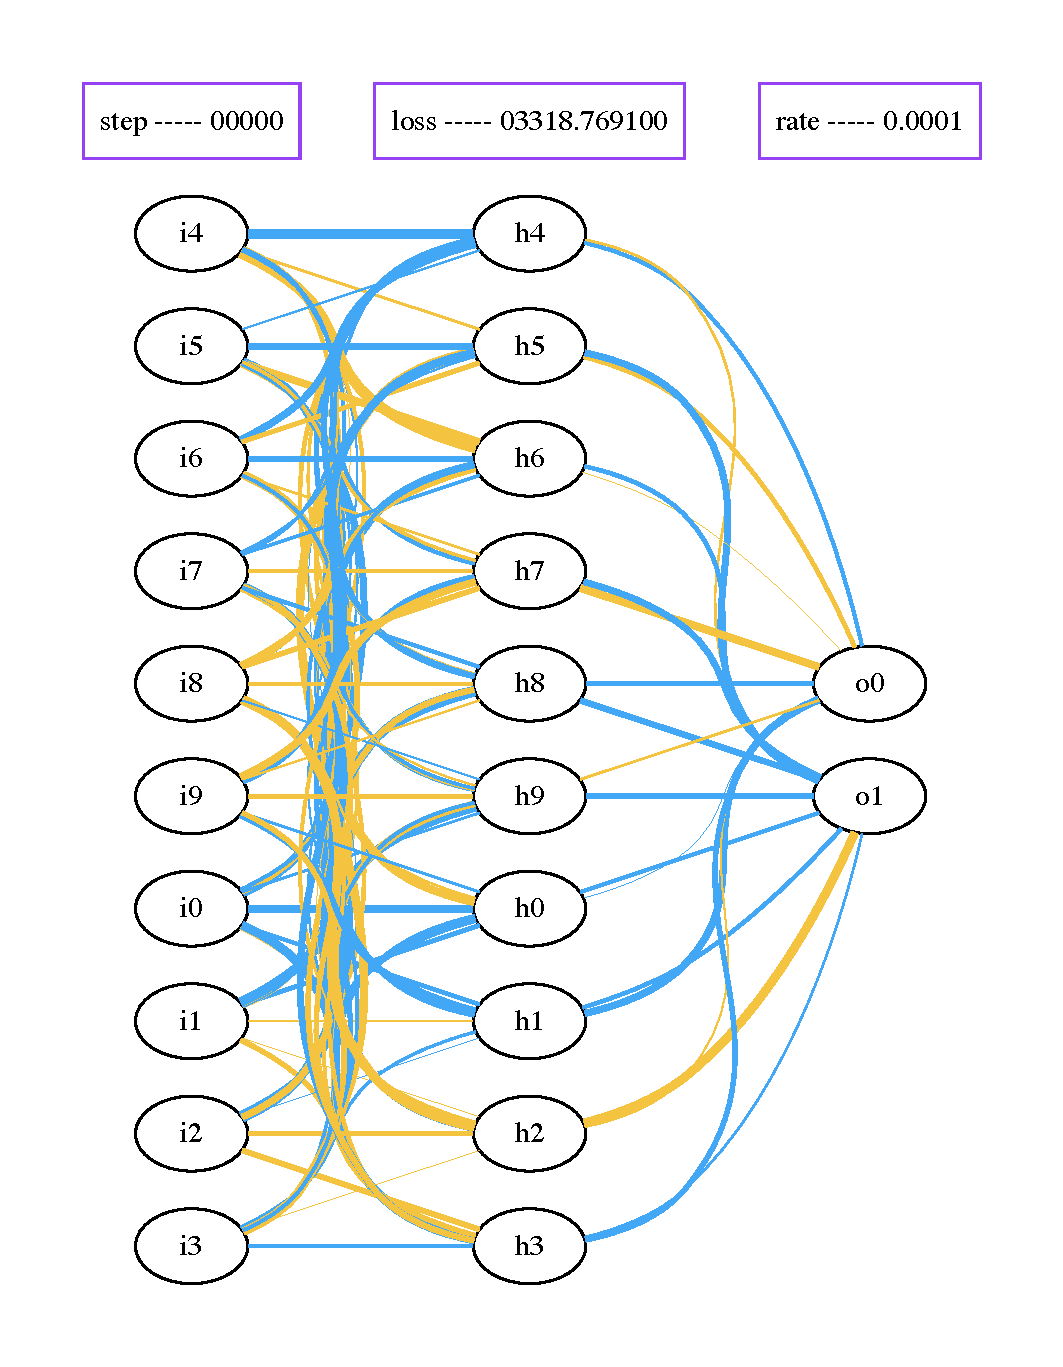
\includegraphics[width=0.3\linewidth]{net_0}
                \label{fig:name}
            \end{figure}
    \end{itemize}
\end{frame}

\begin{frame}
    \begin{itemize}
        \item let $w=[w_{ij}]$ be the matrices of weights between neuron $i$ of
            the left layer and neuron $j$ of the middle layer.
            \begin{equation}
                b_j= \sum^{d}_{k=1}x_kw_{kj} 
            \end{equation}
        \item With $b=(b_1,...,b_m)$ and $x=(x_1,..,x_d)$, we have
            \begin{equation}
                b=xw
            \end{equation}
            \begin{figure}[htpb]
                \centering
                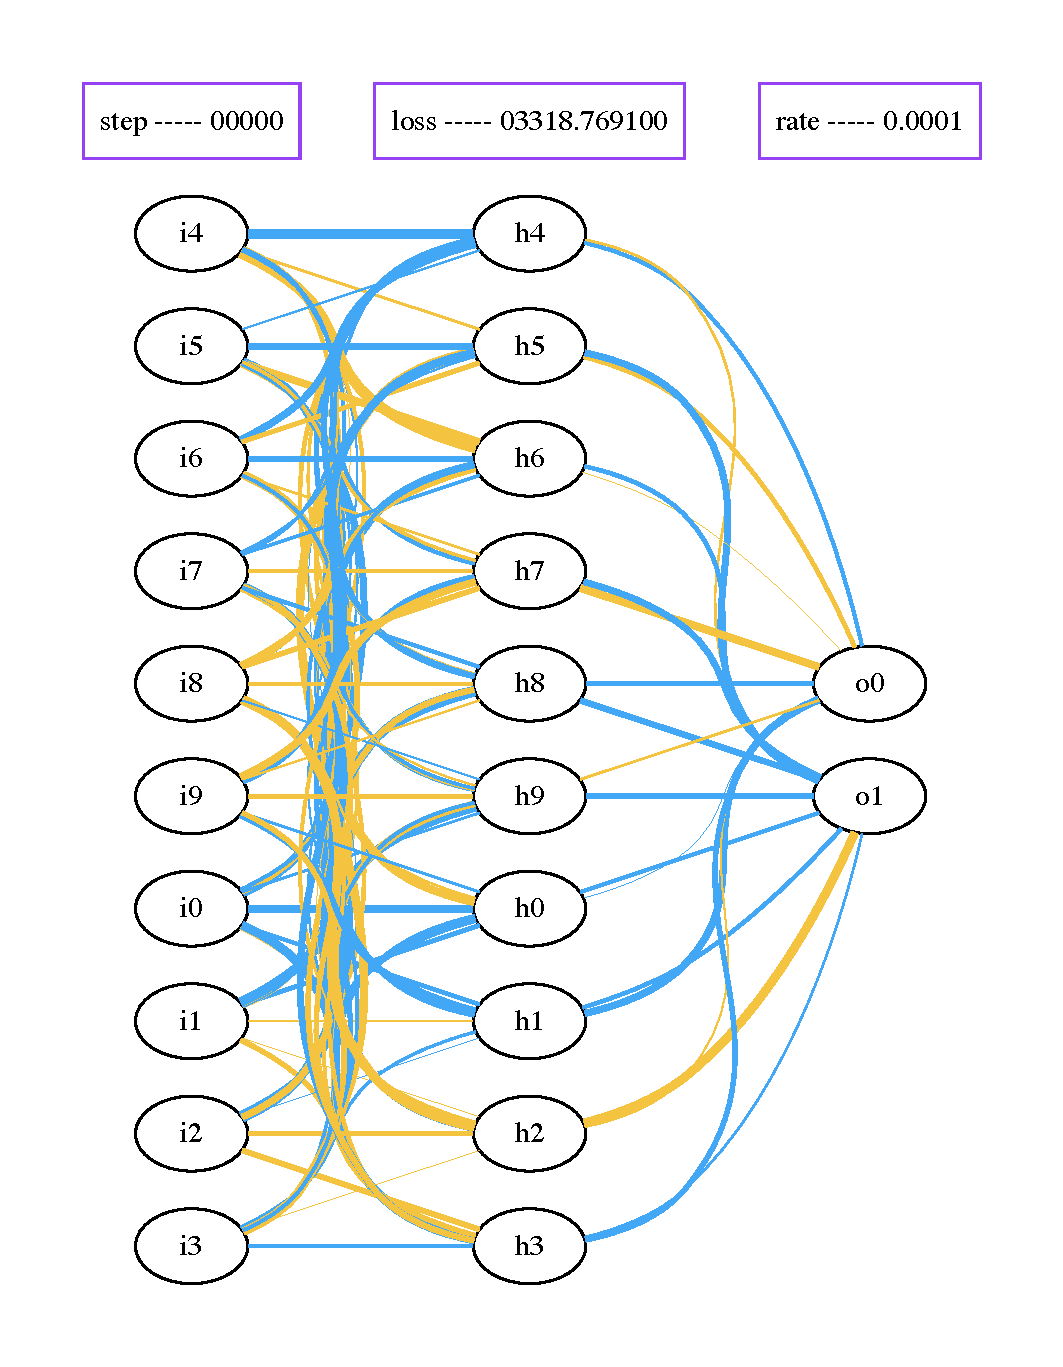
\includegraphics[width=0.1\linewidth]{net_0}
                \label{fig:name}
            \end{figure}
	\item The same notation generalizes to an arbitraty number of input samples ${x_i, i\in[1, n]}$ !
    \end{itemize}
\end{frame}


\begin{frame}{Layers}
    \begin{itemize}
        \item We now know how to compute the input $b$ of a layer as a function of
            the output $x$ of the previous layer  
            \begin{equation}
                b=xw
            \end{equation}
        \item Applying this rule \textbf{{and}} the non linearity $\sigma$, we
            can coompute the \textbf{{forward propagation}} of a neural
            network.
        \begin{figure}[htpb]
            \centering
            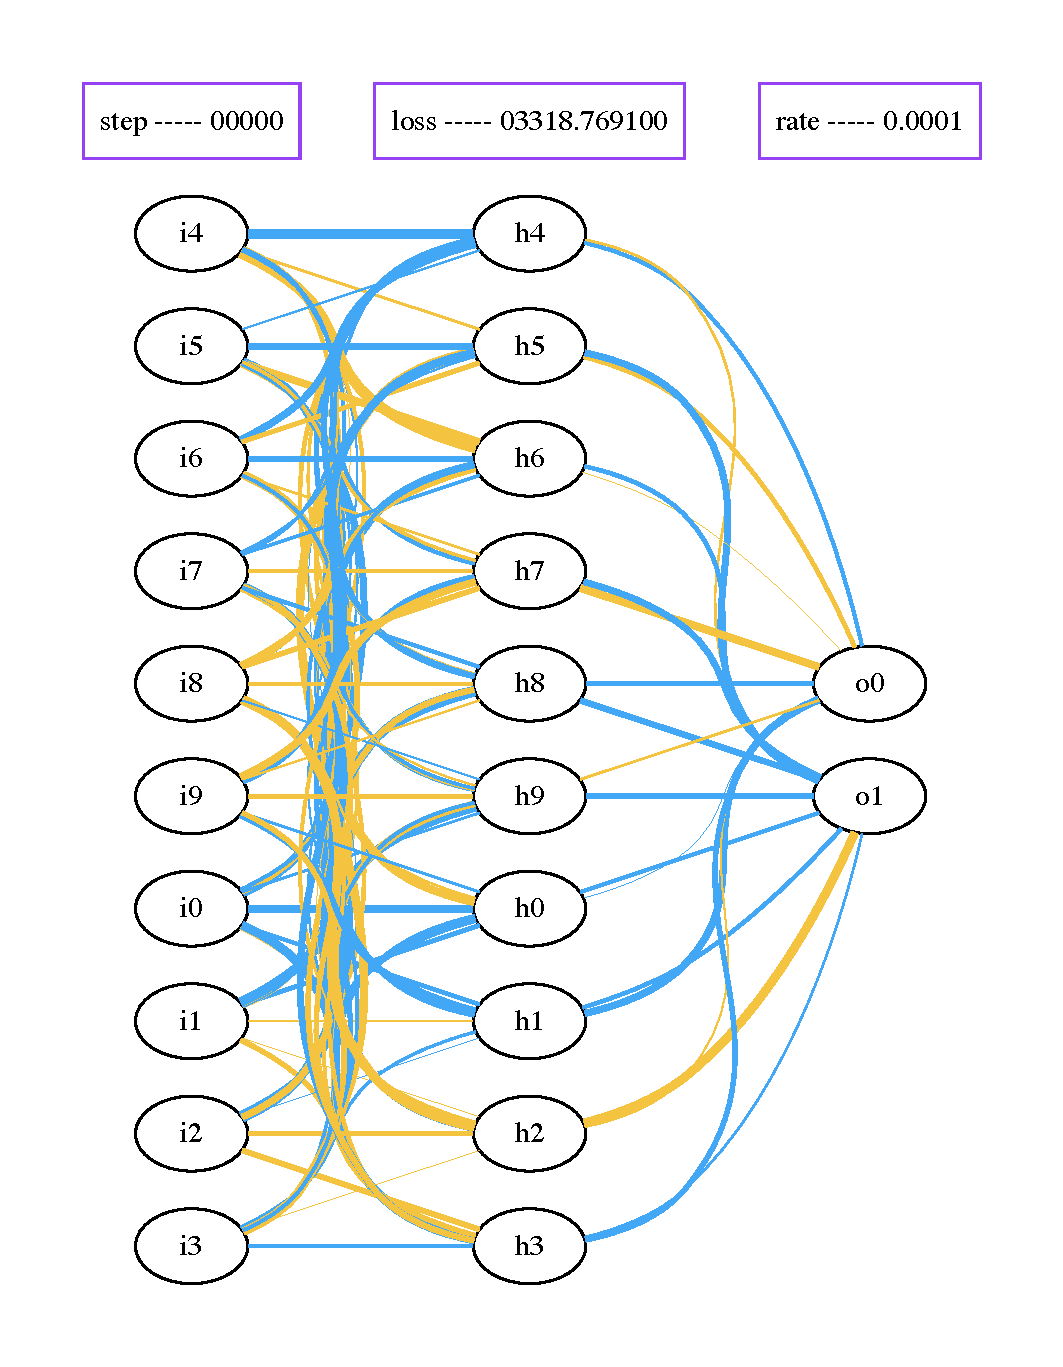
\includegraphics[width=0.3\linewidth]{net_0}
            \label{fig:net_}
        \end{figure}
    \end{itemize}
\end{frame}


\begin{frame}{Layers and forward propagation}
   \begin{itemize}
       \item We will use the \textbf{{numpy}} library to do so.
	\item We will use de ReLu as the non linearity.
   \end{itemize} 
   \begin{figure}[htpb]
       \centering
       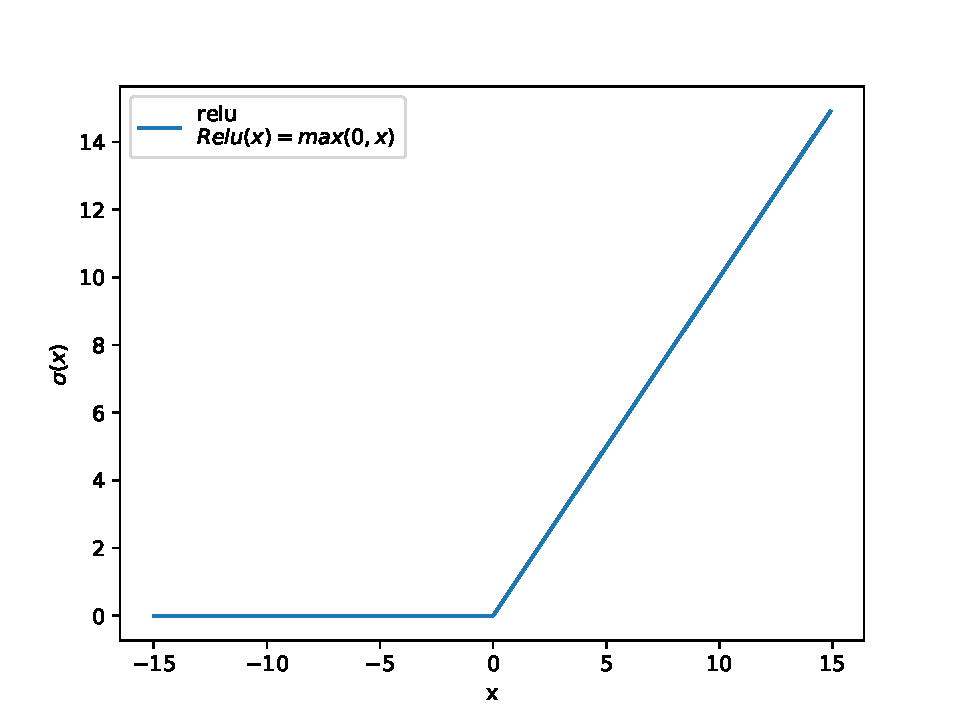
\includegraphics[width=0.5\linewidth]{relu}
       \label{fig:relu}
   \end{figure} 
\end{frame}

\begin{frame}{Relu function}
   \begin{figure}[htpb]
       \centering
       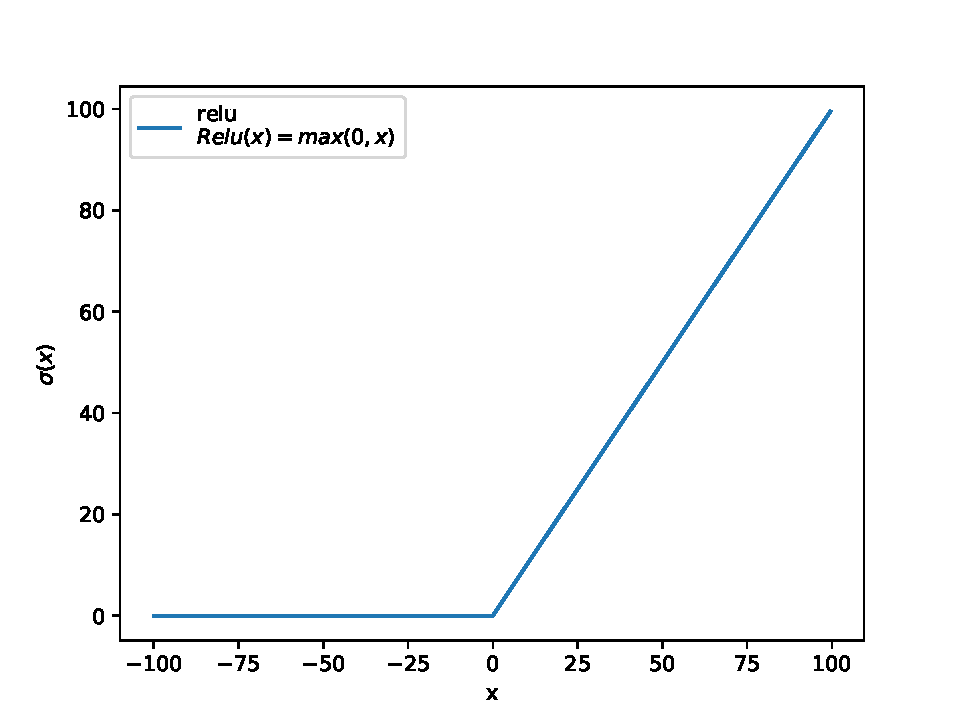
\includegraphics[width=0.8\linewidth]{relu_zoom_out}
       \label{fig:relu}
   \end{figure} 
\end{frame}


\section{Derivation, gradient descent, backpropagation}%
\label{sec:derivation_gradient_descent_backpropagation}


\begin{frame}{Optimization}
    \begin{itemize}
        \item The parameters are the \textbf{{weights}} $w_1$ and $w_2$.
        \item In our examples we will use a network with three layers : input -
            hidden - output.
            \begin{figure}[htpb]
                \centering
                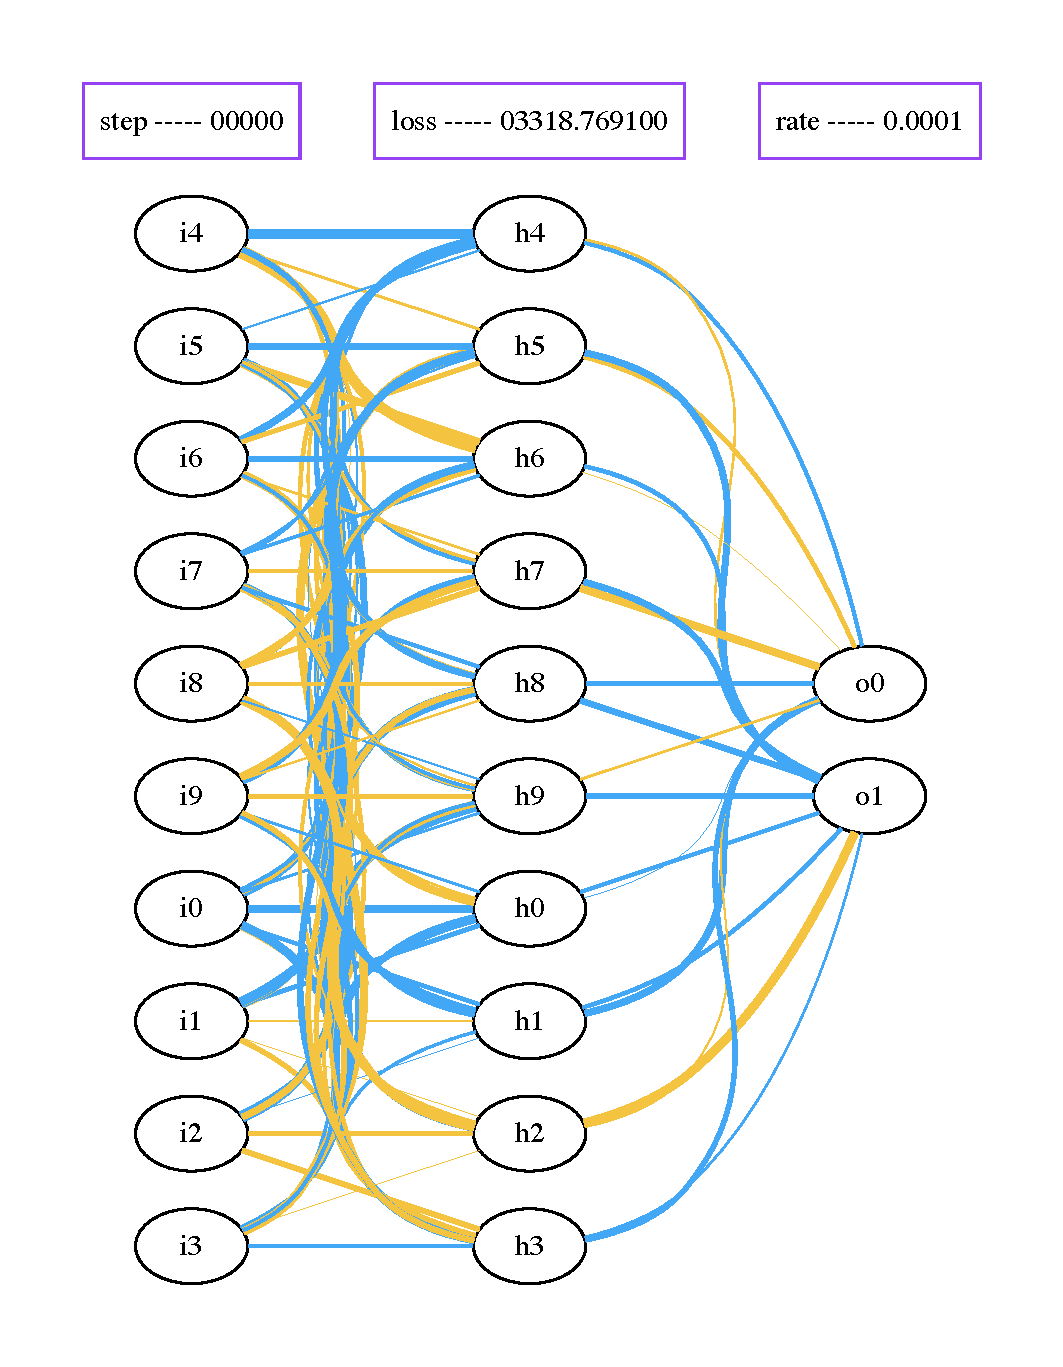
\includegraphics[width=0.3\linewidth]{net_0}
                \label{fig:name}
            \end{figure}
    \end{itemize}
\end{frame}


\begin{frame}{Gradients in a neural network}
   \begin{itemize}
    \item Example of a gradient
        \begin{equation}
            \frac{\partial L}{\partial w1}=  h^T  2(y_{\text{predicted}}-y_{{truth}})  
        \end{equation}
           (where $h$ is the output of the relu)
   \end{itemize} 
\end{frame}


\begin{frame}{Backpropagation}
   \begin{itemize}
       \item By repeating the same process we can also compute the gradient with respect to $w2$.
        \item This is called \textbf{{backpropagation}}.
        \item Knowing the gradient, we can \textbf{{update the network parameters}}.
   \end{itemize} 
\end{frame}

\section{Training and visualizing some neural nets}%
\label{sec:visualizing_some_neural_nets}


\begin{frame}{Learning toy data}
    \exercice{}
    \begin{itemize}
        \item \textbf{cd 2\textunderscore neural\textunderscore networks/toy\textunderscore data \textunderscore
            numpy/}. Some toy data are generated in \textbf{{create\textunderscore data.py}}
	    by a function, + a noise.
        \item You can tune the standard deviation of the noise
        \item Use \textbf{{main\textunderscore train\textunderscore neural\textunderscore
            network.py}} to predict these data by empirical risk minimization.
	\item You will need to experiment with the \textbf{hyperparameters} (defined at the top of the script).
        \item Make the network find a bad local minimum, make it explode
            (overflow), observe the network.
    \end{itemize}
\end{frame}


\begin{frame}{Learning curve}
    \begin{figure}[htpb]
    	\centering
    	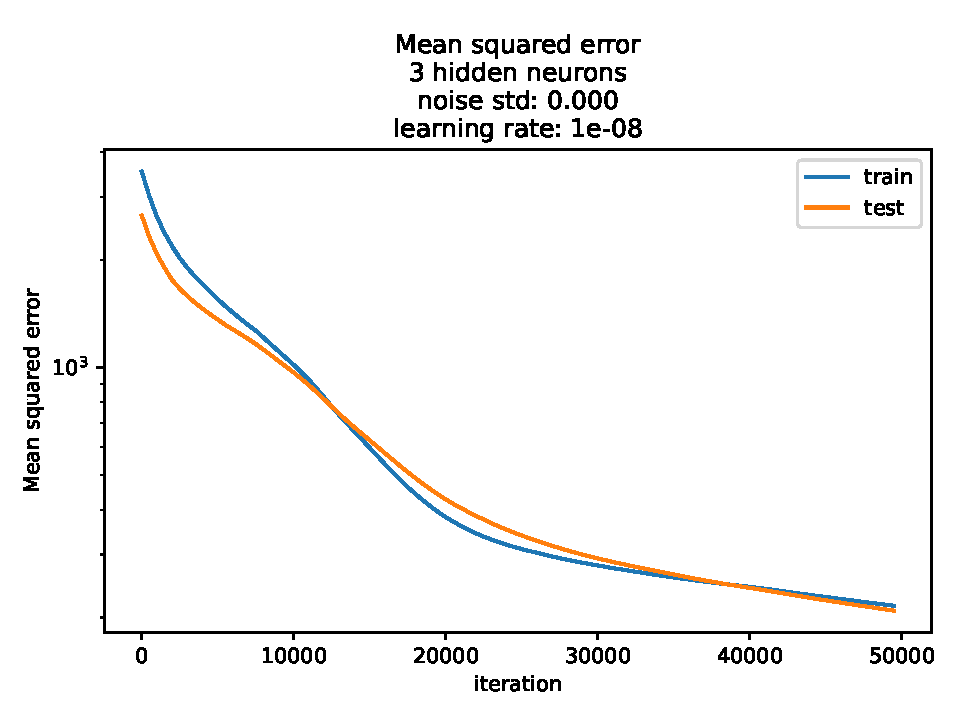
\includegraphics[width=0.8\textwidth]{mse_fun_d_in_6_d_out_2_hidden_3_std_0.0_rate_1e-08}
    	\label{fig:}
    \end{figure}
\end{frame}


\begin{frame}{Learning curve}
    \begin{figure}[htpb]
    	\centering
    	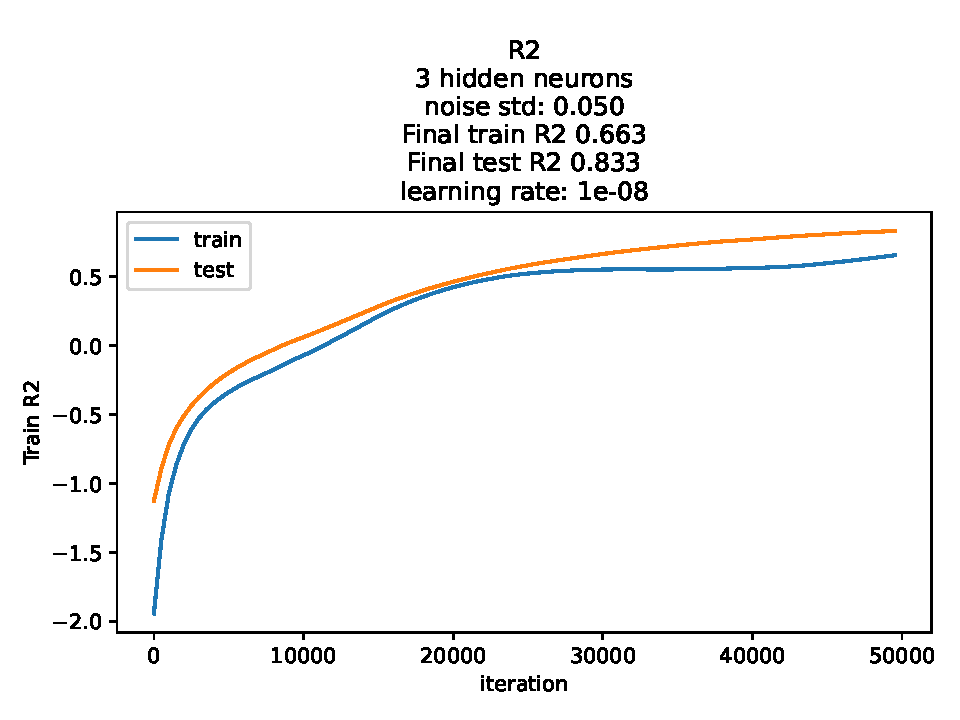
\includegraphics[width=0.8\textwidth]{r2_fun_d_in_6_d_out_2_hidden_3_std_0.05_rate_1e-08}
    	\label{fig:}
    \end{figure}
\end{frame}


\begin{frame}{Learning curve}
    \begin{figure}[htpb]
    	\centering
    	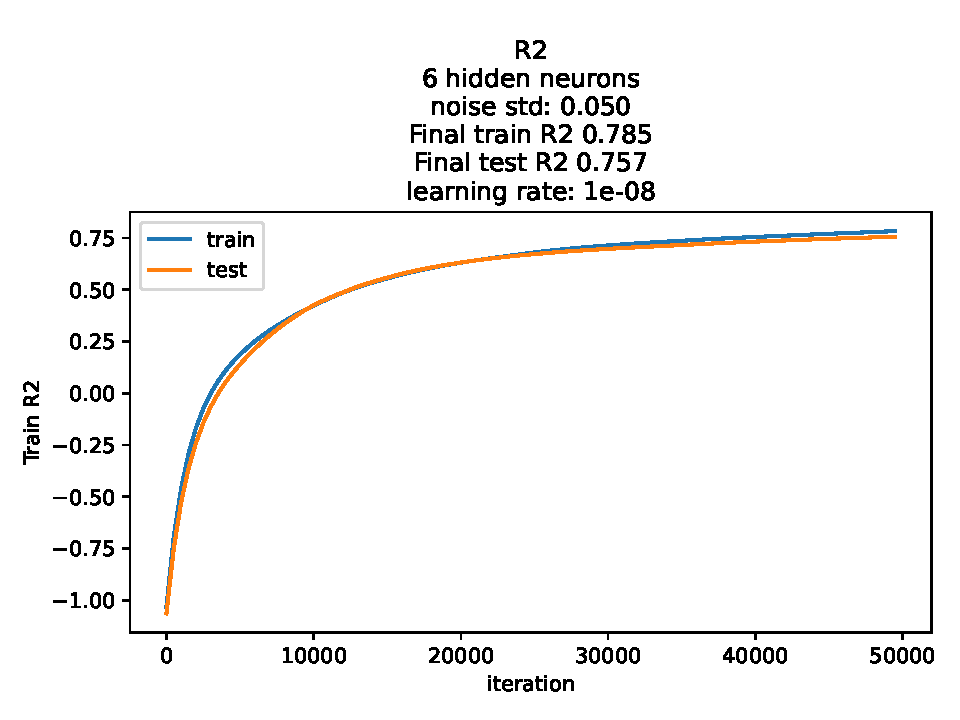
\includegraphics[width=0.8\textwidth]{r2_fun_d_in_6_d_out_2_hidden_6_std_0.05_rate_1e-08}
    	\label{fig:}
    \end{figure}
\end{frame}

\begin{frame}{Plotting}
    \exercice{\textbf{Observation of the network (optional)}}
   \begin{itemize}
       \item  Use \textbf{{plot\textunderscore net}} so
           plot the evolution of the network
        \item You might need to use a smaller network otherwise it will be too
            long.
            \begin{figure}[htpb]
                \centering
                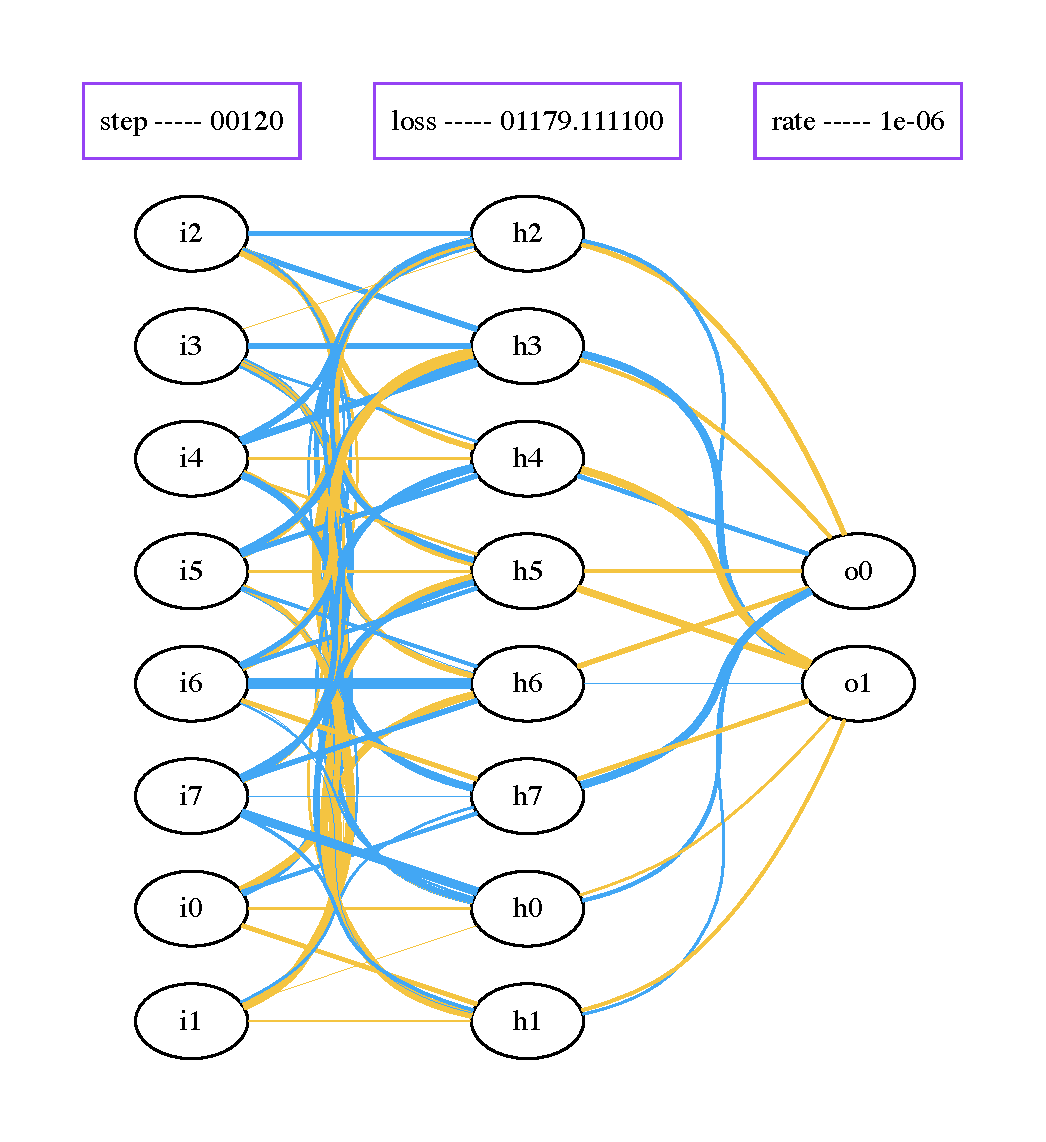
\includegraphics[width=0.4\linewidth]{net_120}
                \caption{}
                \label{fig:}
            \end{figure}
   \end{itemize} 
\end{frame}

\begin{frame}{Initial network}
    \begin{figure}[htpb]
        \centering
        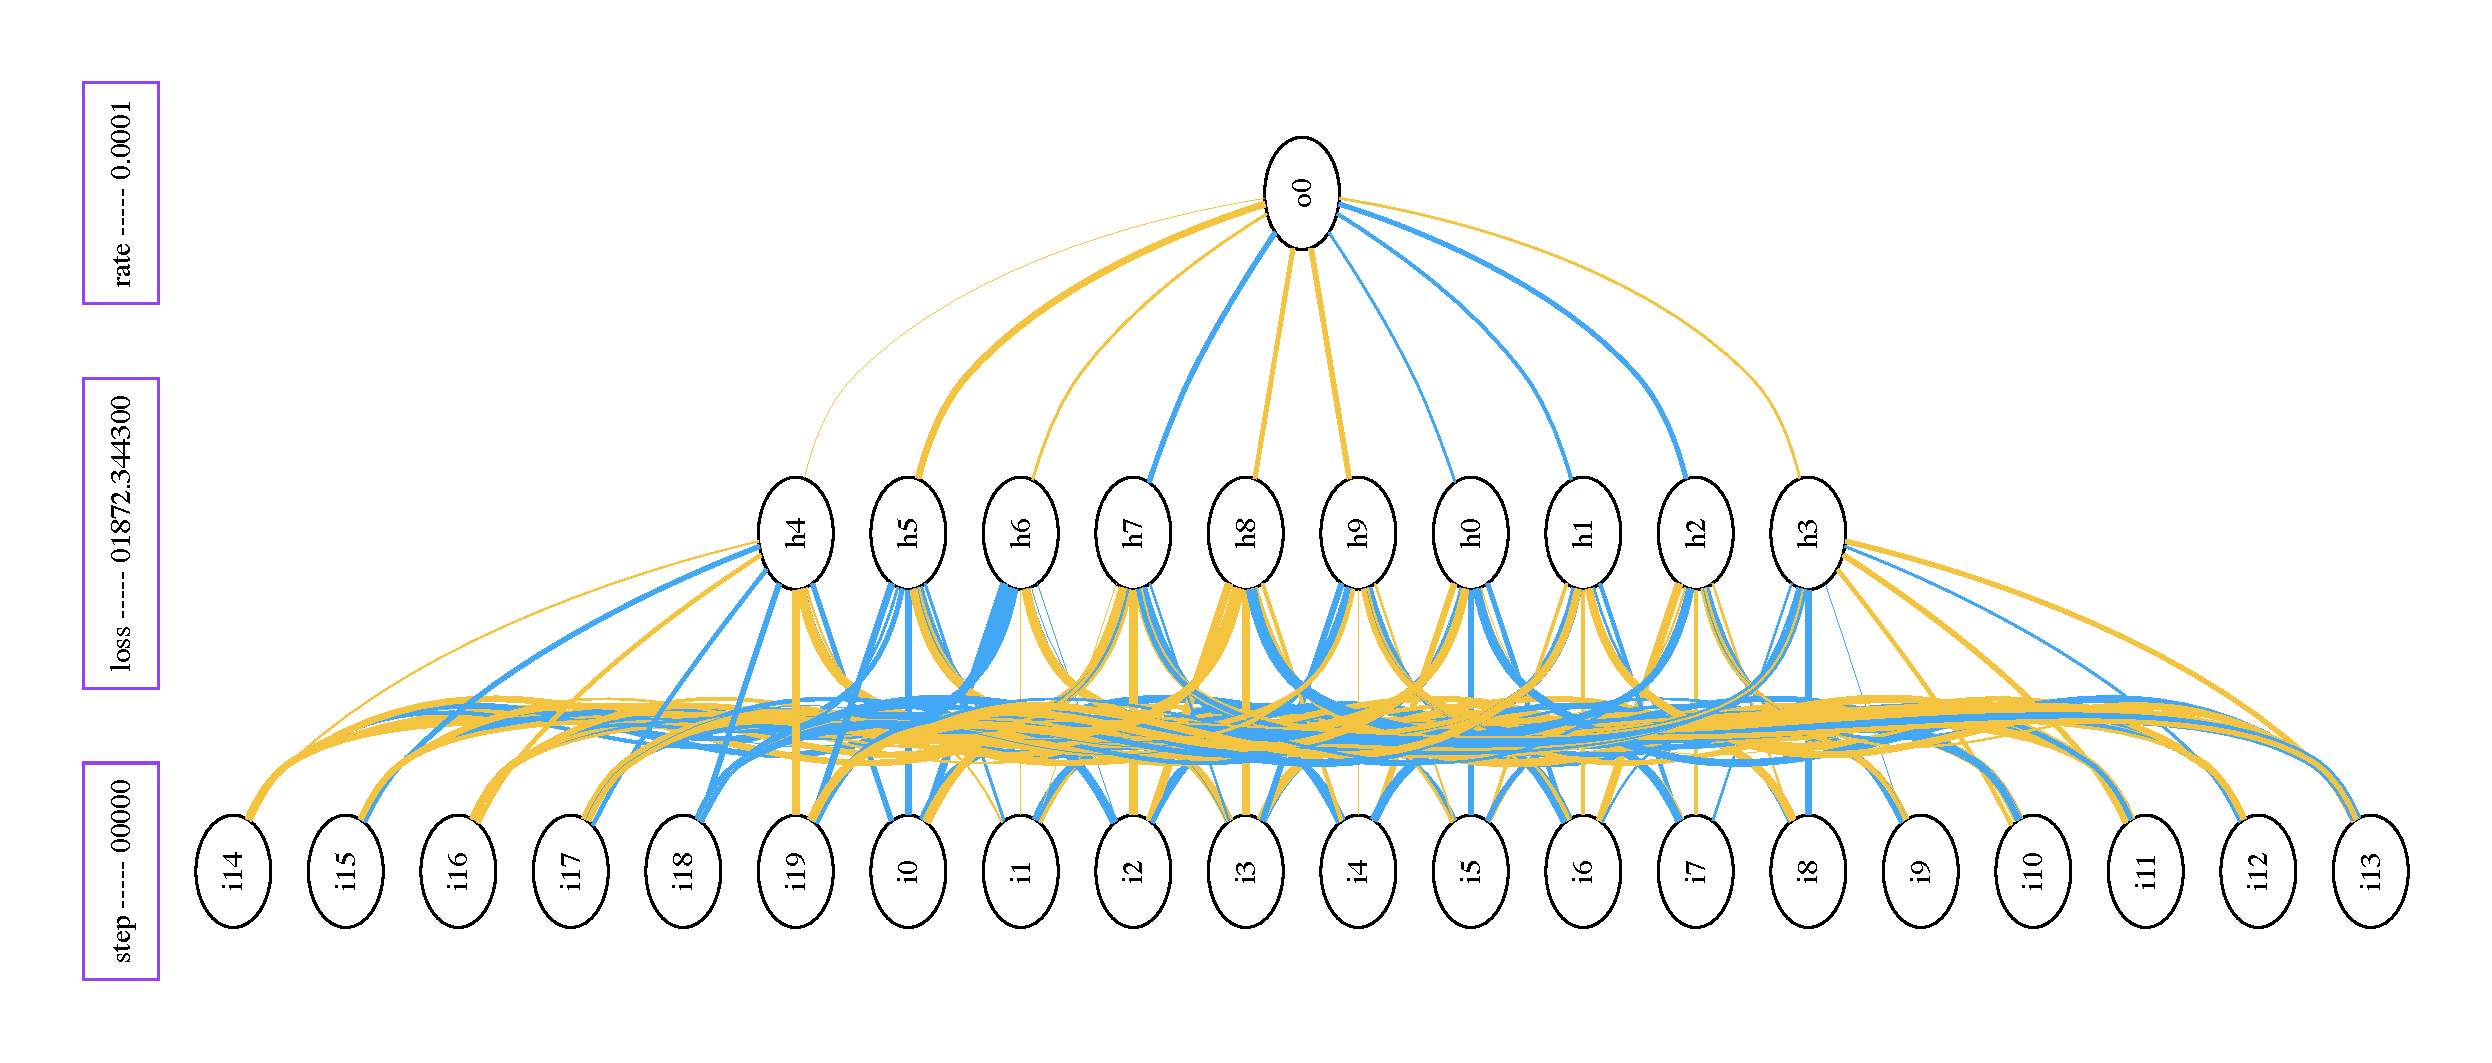
\includegraphics[width=0.9\linewidth]{neto}
        \label{fig:net_0_copie}
    \end{figure}
\end{frame}

\begin{frame}{After 45000 steps}
    \begin{figure}[htpb]
        \centering
        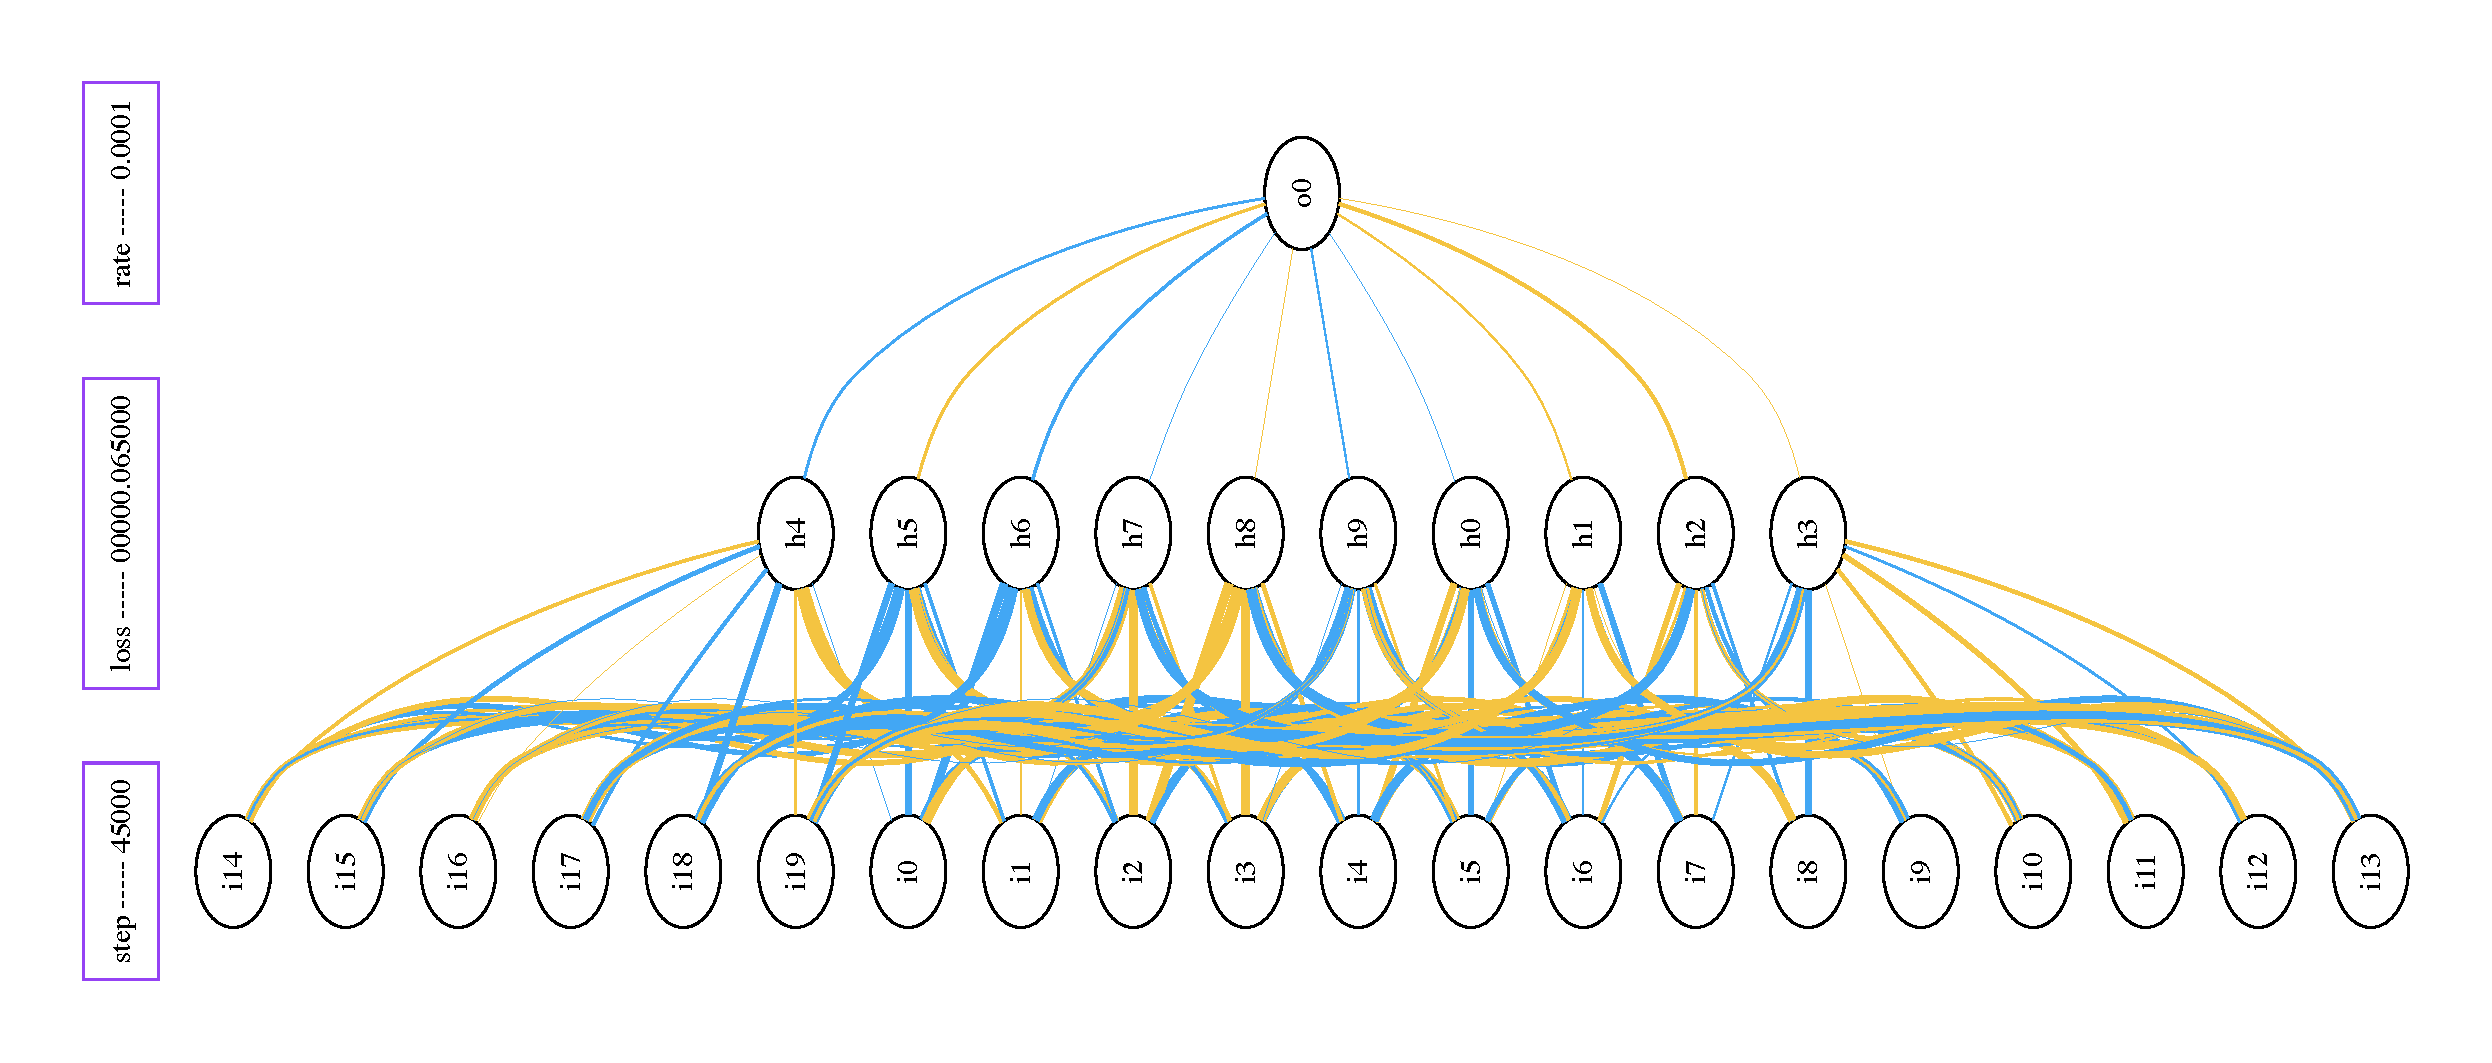
\includegraphics[width=0.8\linewidth]{net_45000}
        \label{fig:net_0_copie}
    \end{figure}
\end{frame}

\begin{frame}{With libs}
    \begin{itemize}
        \item We implemented a neural network manually with numpy, but when the networks are large
            or when we need to automate the seach for good parameters, it is
            more convenient to work with libraries such as :
            \begin{itemize}
                \item pytorch
                \item tensorflow
                \item keras
		\item theano
            \end{itemize}
    \end{itemize}
\end{frame}

\section{Other techniques}%
\label{sec:other_techniques}

\begin{frame}
    \begin{itemize}
        \item There are many specific architectures and methods for neural networks:
            \begin{itemize}
                \item in the number of neurons per layer
                \item type of data processed
                \item relationship between weights (shared weights)
                \item number of hidden layers
                \item recurrent neural networks RNN
                \item convolutional neural networks CNN
                \item graph convolutional networks GCN
            \end{itemize}
    \end{itemize}
\end{frame}

\begin{frame}{Gradient descent}
    \begin{itemize}
        \item Stochastic Gradient Descent (SGD)
        \item Mini-batch learning
        \item Batch learning
    \end{itemize}
\end{frame}


\begin{frame}{Other cost functions}
   \begin{itemize}
       \item Until now we used the squared error cost function
       \item The slowdown problem
       \item The Cross entropy is another possible cost function used
           for classification
   \end{itemize} 
\end{frame}


\section{MNIST}%
\label{sec:jj}

\begin{frame}{MNIST}
    \begin{itemize}
        \item \textbf{cd ../mnist}
    \item We will train a neural network to predicts digits in the MNIST
        database.
    \item With keras and tensorflow, we will achieve an accuracy of more than 97\% in a few minutes for the classification.
    \end{itemize}
\end{frame}

\begin{frame}{Inputs}
   \begin{figure}[htpb]
       \centering
       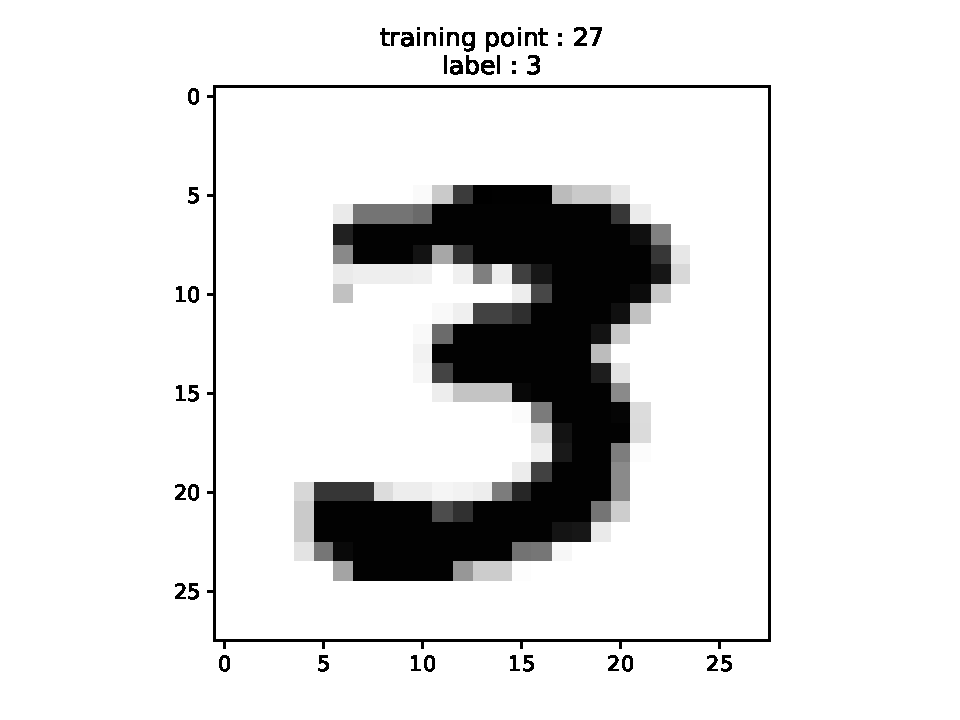
\includegraphics[width=0.7\linewidth]{data_27}
       \caption{Datapoint 27}
       \label{fig:data_27}
   \end{figure} 
\end{frame}


\begin{frame}{Inputs}
   \begin{figure}[htpb]
       \centering
       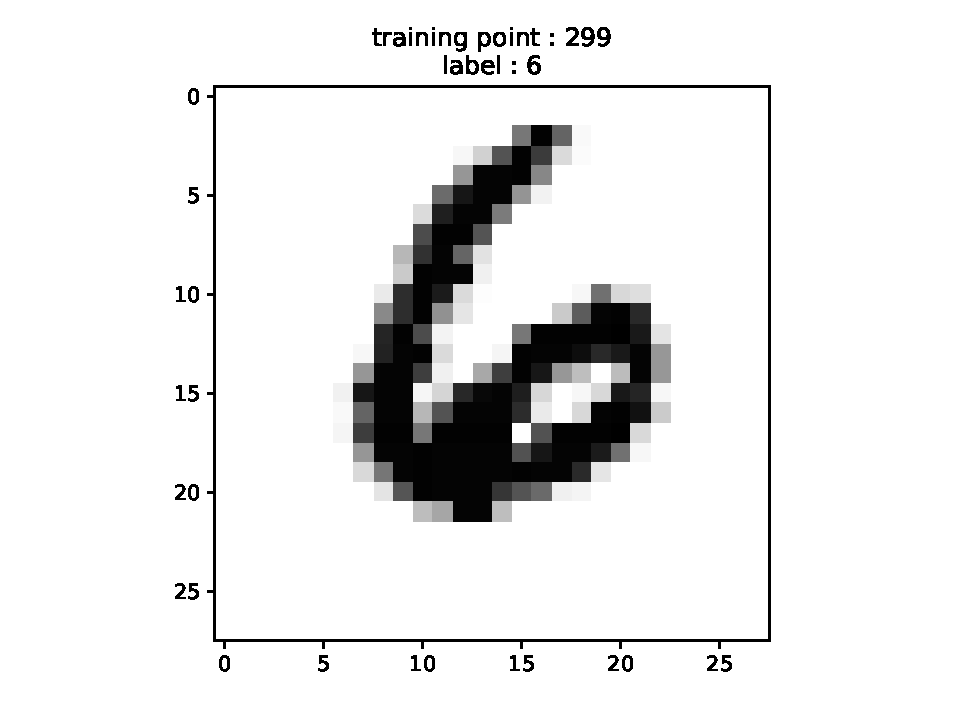
\includegraphics[width=0.7\linewidth]{data_299}
       \caption{Datapoint 299}
       \label{fig:data_27}
   \end{figure} 
\end{frame}



\begin{frame}{Inputs}
   \begin{figure}[htpb]
       \centering
       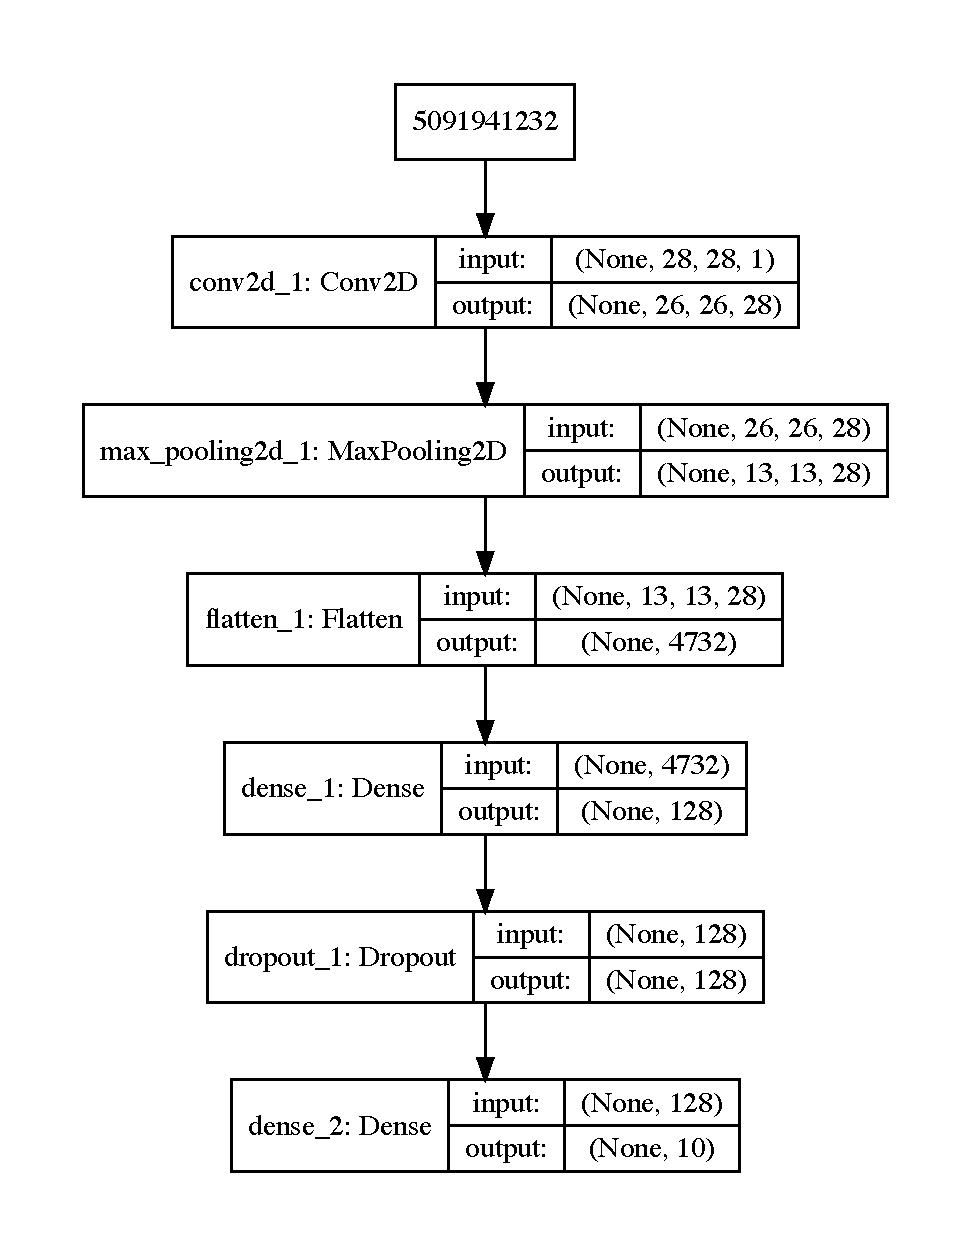
\includegraphics[width=0.45\linewidth]{network_with_shapes}
       \caption{Network shape}
       \label{fig:data_27}
   \end{figure} 
\end{frame}



\begin{frame}{Inputs}
   \begin{figure}[htpb]
       \centering
       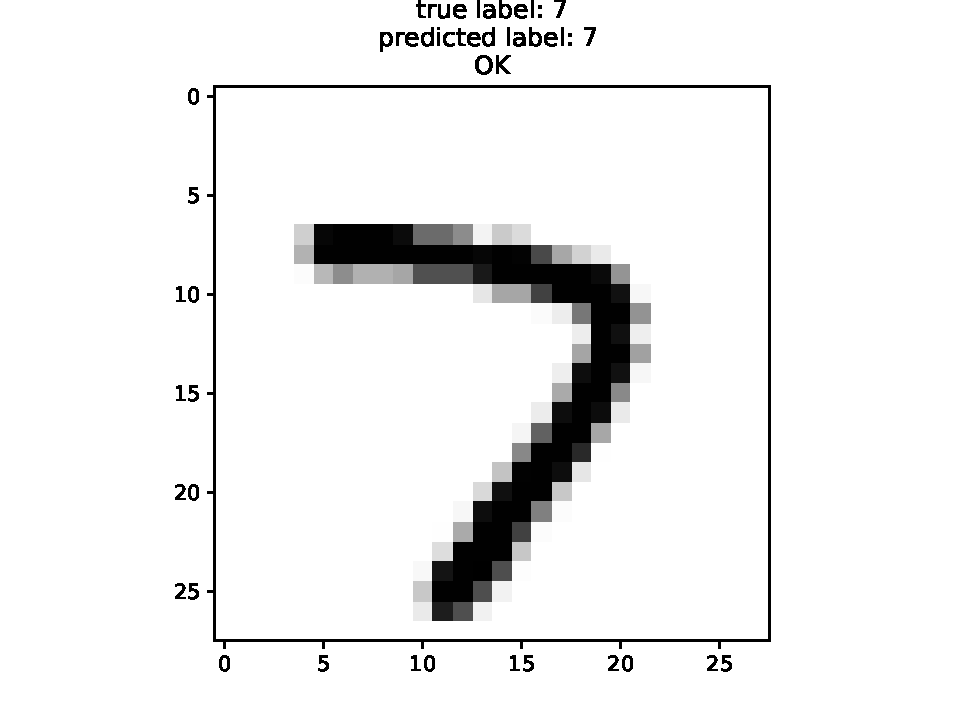
\includegraphics[width=0.7\linewidth]{prediction_17}
       \caption{Predicion for point 17}
       \label{fig:data_27}
   \end{figure} 
\end{frame}


\begin{frame}{Inputs}
   \begin{figure}[htpb]
       \centering
       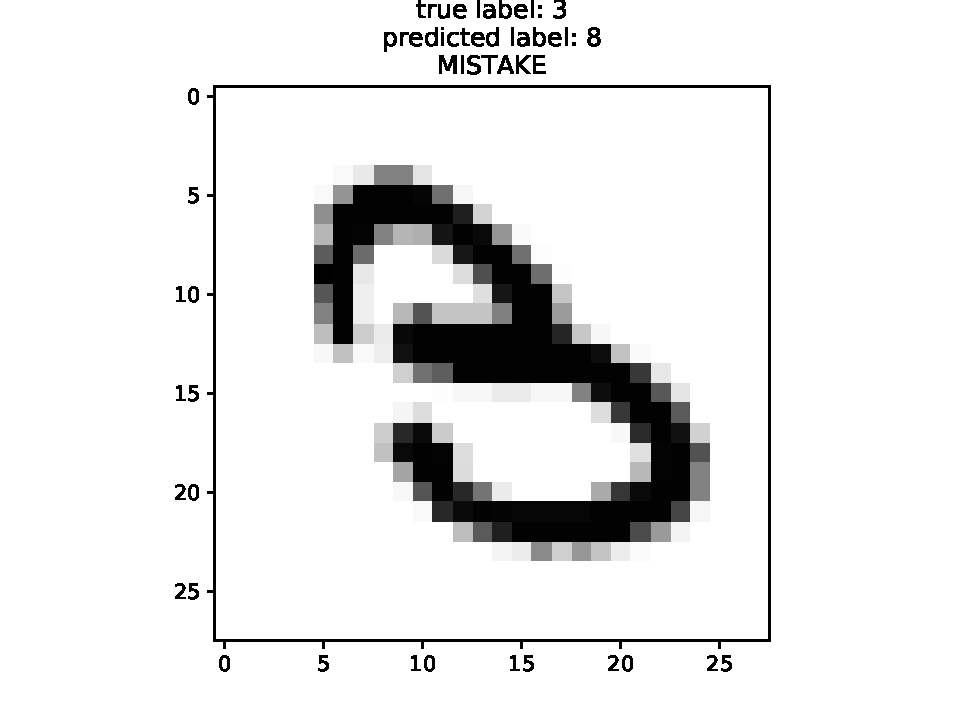
\includegraphics[width=0.7\linewidth]{prediction_18}
       \caption{Prediction for point 18}
       \label{fig:data_27}
   \end{figure} 
\end{frame}

\section{Overparametrization and underparametrization}

\begin{frame}{Underparametrization and overparametrization}

    Neural network have some very specific behaviors in some contexts.

    \url{https://francisbach.com/rethinking-sgd-noise/} 

\end{frame}

\begin{frame}{}
    \begin{figure}[htpb]
        \centering
        
\includegraphics[width=0.8\textwidth]{learning_rates_underparametrized}
    \end{figure}

\end{frame}

\begin{frame}{}
    \begin{figure}[htpb]
        \centering
        
\includegraphics[width=0.8\textwidth]{learning_rates_overparametrized}
    \end{figure}


\end{frame}

\begin{frame}{Double-descent phenomenon and overfitting}

    If optimized correctly, neural networks do not overfit easily !

    This seems to be in contradiction with the classical machine learning
    theory.

    \url{https://arxiv.org/pdf/1812.11118.pdf} 

\end{frame}


\end{document} 
